\documentclass{article}

\usepackage{amsmath}
\usepackage{amssymb}
\usepackage{graphicx}

\begin{document}


Ivan Lin\newline{}
Dr. Esther Arkin\newline{}
AMS301\newline{}
3/19/17

\begin{center}
  Homework 6b
\end{center}

\underline{Problem C}\newline{}
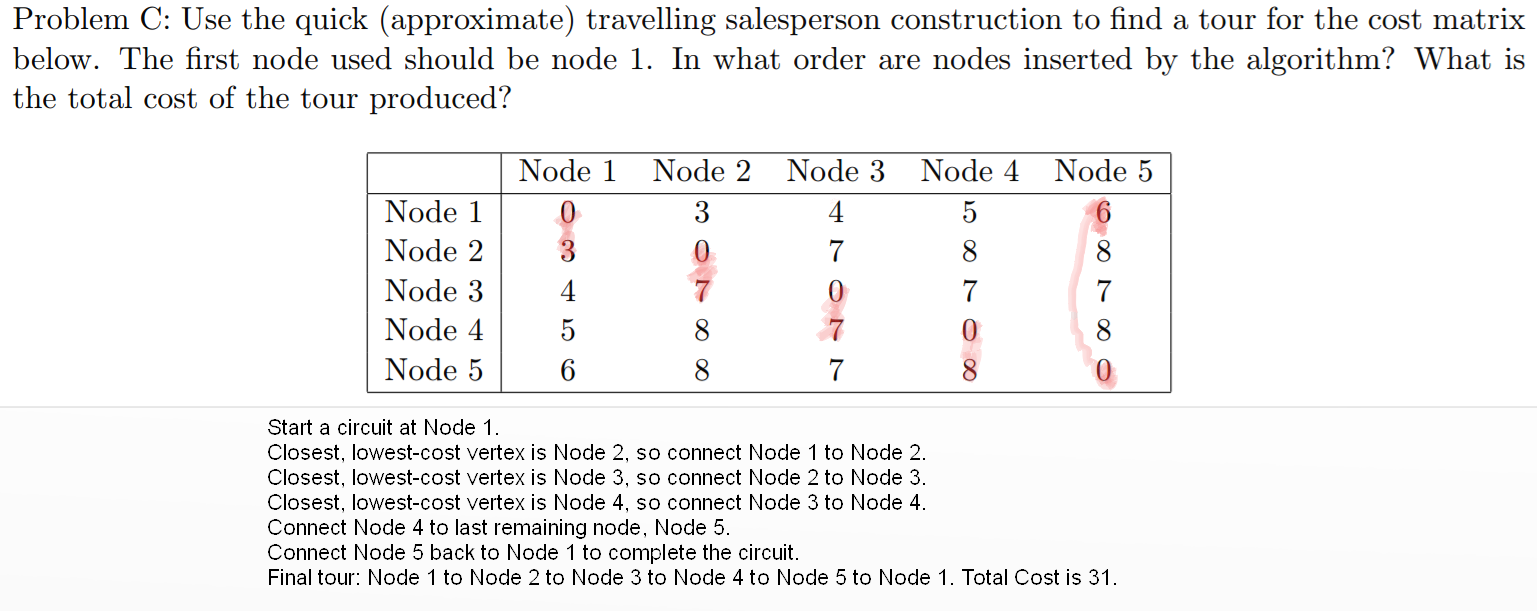
\includegraphics[width=\textwidth]{testams303.png}

\underline{Problem D}\newline{}
I wish to model the following word problem as a graph problem: The Maytag repairman has been called to repair washers and dryers at several customer’s homes. Assume travel times between locations are known. The repairman starts and ends his day at his home, and would like to complete his work as quickly as possible.\newline{}
(a). What do the nodes of the graph to be constructed represent?\newline{}
The nodes of the graph represent the customers' homes that the repairman needs to visit.\newline{}
(b). What do the edges of the graph to be constructed represent?\newline{}
The edges of the graph represent the trips between the homes. The costs of the edge would represent the travel time of the trips.\newline{} 
(c). State which graph problem it is: Shortest path, Minimum spanning tree, Traveling Salesman Problem,
Breadth or Depth First Search\newline{}
This model is essentially a variation of the Travelling Salesman Problem.\newline{}

\underline{Problem E}\newline{}
For each of the following parts, state True or False. If true, give a short proof. If false, giver a
counterexample. We are given a connected graph G with costs on edges. Assume all costs are positive and
that there are no ties. A, B are nodes in the graph.\newline{}
(1). If an edge e is part of a Minimum Spanning Tree then it cannot be part of a Maximum Spanning Tree. \textit{False. See counterexample below.}\newline{}
(2). If an edge e is part of a Shortest Path Tree rooted at A then it must also be part of a Shortest Path
Tree rooted at B. \textit{False. See counterexample below.}\newline{}
(3). If all edge costs are multiplied by 2 the Shortest Path Tree rooted at A remains the same tree.
\newline{}
\textit{True.} Let $P_1=e_a+e_b+...$ represent a path on the shortest path tree rooted at A. Let $P_2=e_x+e_y+...$ represent any alternative paths on the tree between the two same endpoints. By multiplying all edges on the graph by a positive constant $k$, the cost of those paths. The cost of $P_1'$ is $kP_1=ke_a+ke_b+...$ and the cost of $P_2'$ is $kP_2=ke_x+ke_y+...$ since the constant can be factored out. So the cost of $P_1'$ will still be less than the modified costs of all other paths, meaning all paths will remain part of the new shortest path tree.
\newline{}
(4). An edge e whose cost is the largest in the graph can not be part of a Shortest Path Tree. \textit{False. See counterexample below}\newline{}
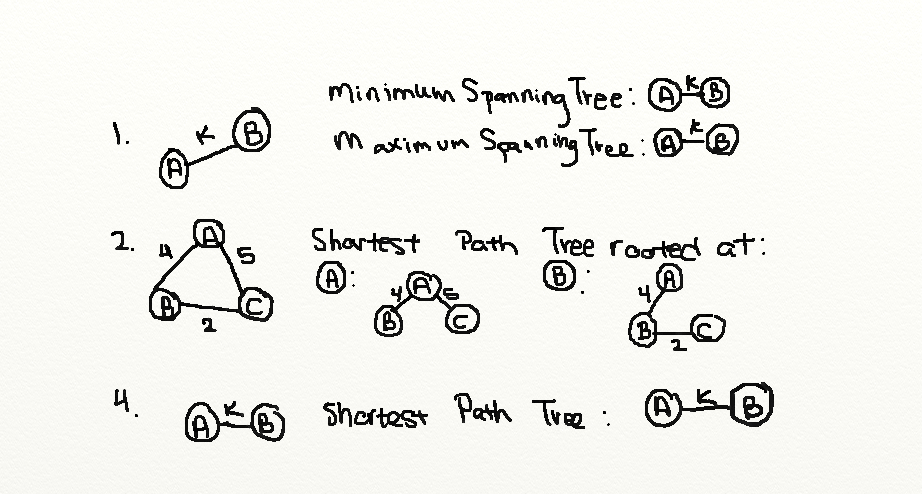
\includegraphics[width=\textwidth]{testams304.png}

\end{document}
